\chapter{Social Routing Client Application}
The Social Routing Client is composed by four major components, each with it's own compromise and objective.
The Activities\cite{activities} and Fragments\cite{fragments} to represent the User Interface (UI) where the user can interact with
the application, the View Models\cite{viewmodel} to store
and manage UI related data, a Repository that handles data operations and knows where to retrieve data from and a 
Remote Data Source to communicate with external components, for instance the Social Routing API or the Google Sign-In API\cite{googlesignindocs}. 
This logic is represented in the figure \ref{fig:clientarchitecture}.

\begin{figure}[h]            
        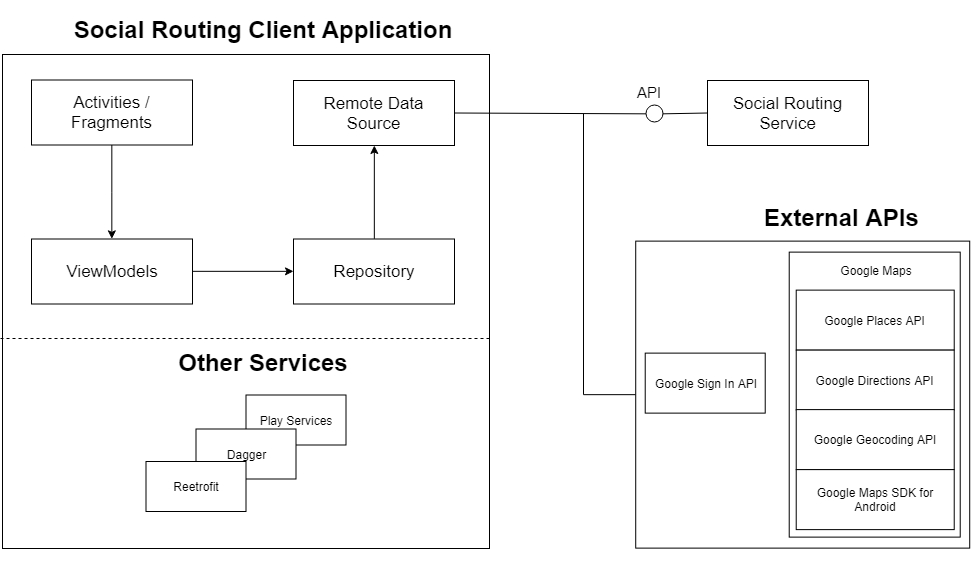
\includegraphics[width=\textwidth]{images/project-structure/social-routing-client-application-structure.PNG}
        \caption{Social Routing Client architecture.}
        \label{fig:clientarchitecture}
\end{figure}
\newpage
\section*{Activities/Fragments}
The concern of this component is to provide a way for the user to interact with the application.
All activities extend a BaseActivity that has a global behavior such as when the data is changed and is necessary to update the view.\\

Each Activity has its own :
\begin{itemize}
        \item Design: defined by one or more layouts that contains buttons, images, input text, fragments (for instance the map fragment provided by Google), with which the user can interact.
        \item Behavior: when the data changes the view needs to be updated, behavior this, that is defined with either a success or error, using the ViewModel.
\end{itemize}
 
An example activity is the NavigationActivity where the user can navigate to all the functionalities of the application, after google authentication, like the creation of a route, 
search or the user profile. This activity haves a left panel where you can navigate to other activities with different purposes such as route creation or the user profile. 
However the activity itself has the search functionality, where you can input the location name that is pretended and a button to navigate to the activity that shows the 
results of that search.

\section*{View Models}
Component used when the UI experiences a change. The View Model calls
other components to load the data, and it can forward user requests to
modify the data however it doesn't know about UI components, 
it is completely separated from them. \\
This component has a simple implementation, the application contains two View Models one for the Routes information (get, creation, update, search) and the other 
to the User (get, delete). It uses the repository to obtain the data and then return it in the shape of Livedata\cite{livedata}.

\section*{Repository}
The Repository Handles data operations, knows where to get the data from
and what API calls to make when the data is updated. A repository can be
considered a mediator between different data sources, such as web services. \\
The application has a repository specified to the Social Routing API and another to Google Maps API\cite{googlemaps}. Each one as correspondent Web Service that uses the
framework Retrofit\cite{retrofit}, used to make a synchronous or asynchronous HTTP request to the remote webserver. The Repository obtains the data
from the web server and can only have two possible request status: Failure or Success. It returns the data contained in a LiveData because when the data 
updates can then be observable. \\
The Repository specific to our API (Social Routing API) knows all the endpoints that should make the request, depending on the objective and the functionality, like 
the endpoints to sign in, to get user info, routes, create a route, get all categories, update a route, amongst others. \\
On the other hand the other repository is used to make request to the Google Webserver (Google Maps API) about the geocode of a location and the directions to a coordinate in the map. 

\section*{Remote Data Source}
Module that has the objective of communicating with external APIs which it does by executing requests to either the Social Routing API, the Google Maps API or the Google Sign-In API. 
The Component knows the structure of the HTTP request to the endpoints, like the parameters and meta-data necessary to obtain the required Response.
After the request is done, the webservers provide the response in the Json\cite{jsonwebsite} format, however the response is deserialized using the library Jackson\cite{jackson},
to convert it to Object. So was defined all the input model objects, to automatically deserialize the response to object.\\

The Client Application has the minimum API level 19 and the target API level is 28, so the Platform version is the Android 9.
It uses Kotlin as the only the programming language in the project which is an object oriented programming language. 
The goal was to improve the coding experience in a way that was practical and effectual. Kotlin is entirely compatible with Java and was specifically designed
to improve existing Java models by offering solutions to API design deficiencies. \\
The core functionalities of the application require a map to create the routes and to show them which was done was using the Google Maps API.
All the functionalities of the application are provided from de Social Routing Service, except all that is related to the Google Maps. All the information is obtained from the server by doing
requests to the correspondent endpoint and it is always necessary to send either the token created by the server or the Google Sign-In API tokenId, used on the user registration process.
The requests that are related to location retrieval or Map UI require a specific request to the Google Maps API. \\
\newpage
\section*{Use Case}
As an example, the user first experience flow of the application is the following:
        \begin{itemize}
                \item The user provides his google account credentials to authenticate with the application, which in its turn makes a request to the backend server.
                \item The user will be redirected to a navigation screen that contains a route search bar and a left panel menu with buttons to redirect to the screens of user profile and route creation.
                \item After the user searches routes using a location, a redirection to a new screen occurs in which a list of found routes is shown.
                \item Once a route is chosen and pressed upon, a new activity with a map is shown, where the route is represented and with a button to start Live Tracking.
                \item By choosing to start Live Tracking the user location is now showed as well as a path to reach the beginning of the chosen route.
                \item If the user wants to see the his profile he may go back until the navigation screen and click in the left panel and then in the User Profile button.
                \item In the user profile the user information (user rating, name, email and routes created) is shown.
                \item For creating a route, a button press in the bar menu is required.
                \item This action takes the user to a new screen that shows the map, a button to finish and a form, asking the location of the route that will be created.
                \item The user must then insert the location on which the map will zoom in.
                \item A click in the map will add the pressed location point to the route being created. If something wrong occurs the user can delete the last point of the route clicking the button on the top of the screen.
                \item When finished the user click in the button to fill the final form that contains the name, description and category of the route.
        \end{itemize}